%!TEX root = ../dokumentation.tex

\chapter{Server}
\label{ch:Server}

Der Befehl \glqq npm run dev\grqq{}, der auch in der \glqq package.json\grqq{} (vgl. autoref{ch:package.json}) beschrieben ist und der innerhalb des Dockerfiles aufgerufen wird, startet den Node-Server. Dafür wird per \glqq nodemon\grqq{} die Datei \glqq server.js\grqq{} angesprochen, welche sodann den Server auf Port 3000 startet.

\begin{figure}[h]
\centering
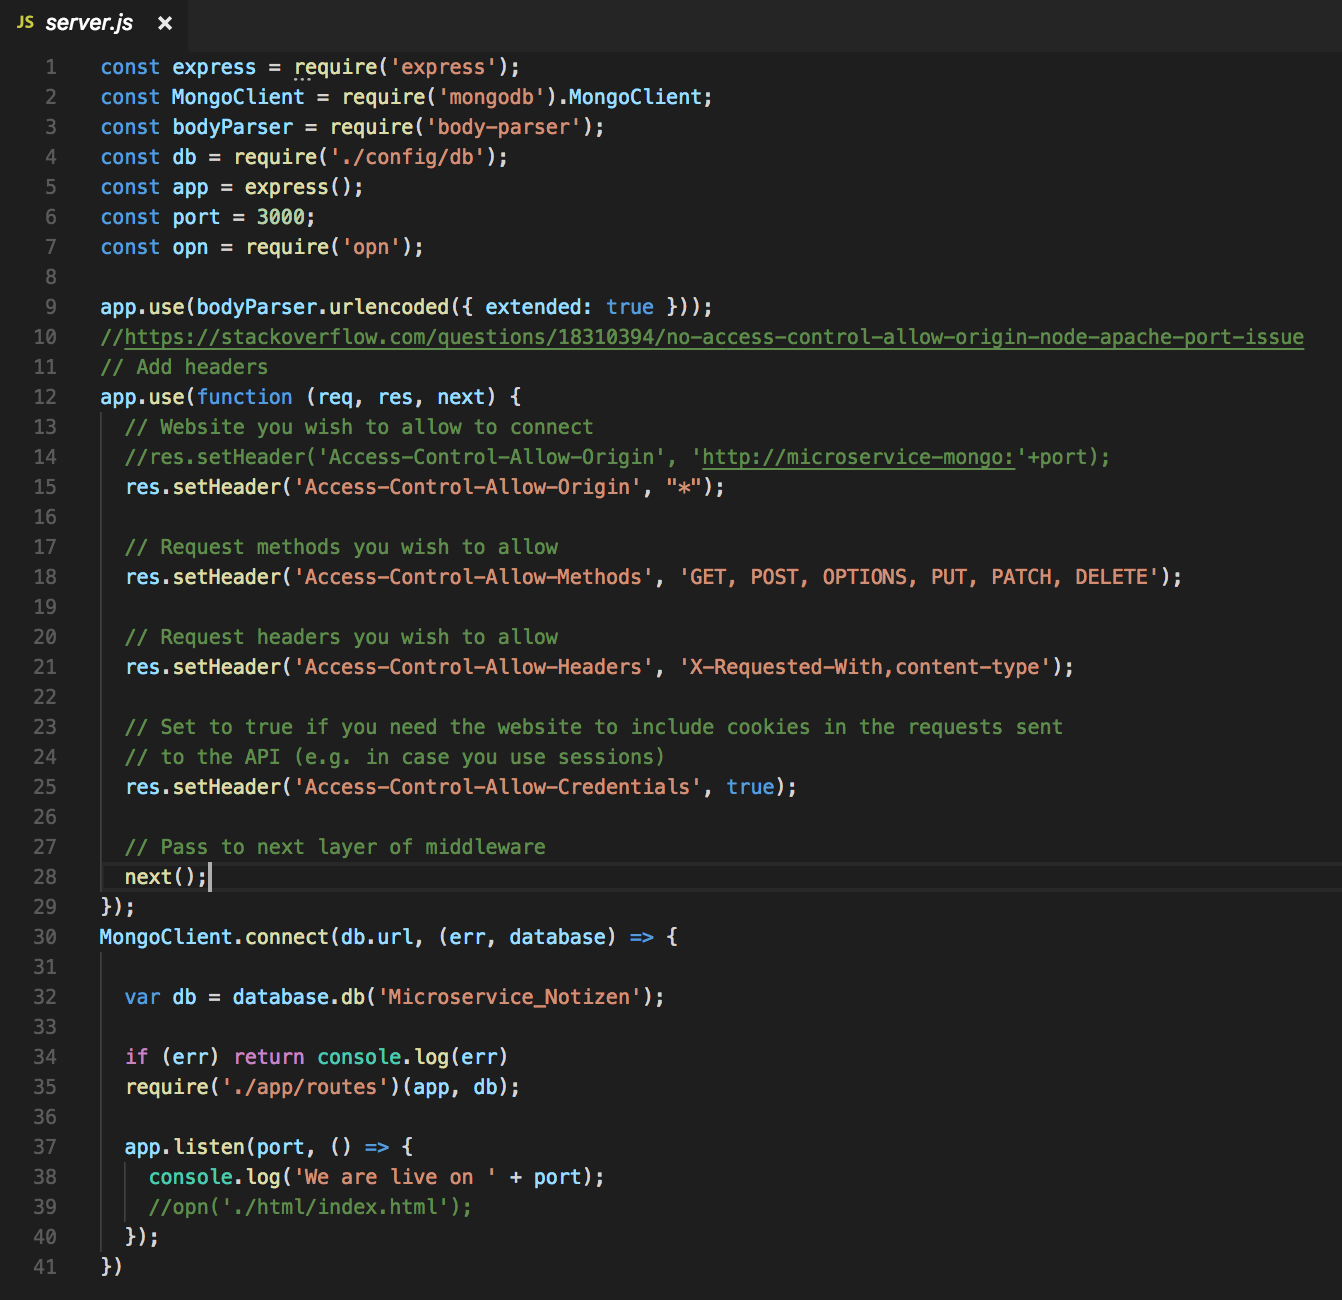
\includegraphics[height=0.9\textwidth]{ServerMain.png}
\vspace{1pt}
\caption{server.js des Node-Servers}
\label{fig:server.js des Node-Servers}
\end{figure}


In den Imports innerhalb der oberen Zeilen 1 bis 7 werden die benötigten Module geladen und dem Server zur Verfügung gestellt.

Die darauffolgenden Zeilen 9 bis 29 werden vom \glqq BodyParser\grqq{} benötigt und liefern die benötigten Daten zur Verarbeitung von Requestbodies.

Ab Zeile 30 wird der Node-Server definiert. Dafür wird die Datenbankverbindung definiert, der Import der Routes vollzogen und dem Server mitgeteilt auf welche Ports er hört und wie er das Empfangene anhand der Routes verarbeiten soll.